\documentclass[10pt,twocolumn,letterpaper]{article}

\usepackage{iccv}
\usepackage{times}
\usepackage{epsfig}
\usepackage{graphicx}
\usepackage{amsmath}
\usepackage{amssymb}
\usepackage[numbers,compress]{natbib}
\usepackage{booktabs}

% Include other packages here, before hyperref.

% If you comment hyperref and then uncomment it, you should delete
% egpaper.aux before re-running latex.  (Or just hit 'q' on the first latex
% run, let it finish, and you should be clear).
\usepackage[pagebackref=true,breaklinks=true,letterpaper=true,colorlinks,bookmarks=false,colorlinks=true,allcolors=blue]{hyperref}


 \iccvfinalcopy % *** Uncomment this line for the final submission

% Pages are numbered in submission mode, and unnumbered in camera-ready
\ificcvfinal\pagestyle{empty}\fi

\begin{document}

%%%%%%%%% TITLE
\title{UCF CAP 5516 Project Proposal}

\author{Ronald Campos\\
MSCV Program\\
{\tt\small roncamposj@knights.ucf.edu}
\and
Suneet Tipirneni\\
MSCV Program\\
{\tt\small  suneet.tipirneni@knights.ucf.edu}
}

\maketitle
% Remove page # from the first page of camera-ready.
\ificcvfinal\thispagestyle{empty}\fi


\begin{abstract}
    As healthcare becomes more democratized, the need to validate potential harmful substances has become more and more important. This is especially true when it comes to medications. We want to propose an alternative way to identify pills by developing
    a model for identifying pills that relies on the robust and modern transformer architecture.
\end{abstract}


\section{Problem Definition}
Given an input of an image, our goal is to identity and provide a text output for pills/medications in the image. Having more tools to identify potentially hazardous substances can lead to safer environments especially in the pharmaceutical domain. The end goal of this project is to enable people with a non-pharmaceutical background the ability to identify pills/medications with ease using computer vision.

\section{Related Work}

Our related work is primarily comprised of the existing knowledge of vision transformers and the original paper
that performed pill identification using a CNN-like architecture.
\begin{itemize}
    \item An Image is Worth 16x16 Words: Transformers for Image Recognition at Scale~\cite{an_imageworth}
        \item A Low-Shot Fine-Grained Benchmark for Pill Identification~\cite{ePill}
\end{itemize}

\section{Dataset}
We will be using the ePillID dataset~\cite{ePill} for this work.  This dataset contains $13,000$ images and $4,902$ different pills.  There are $9,804$ different classes in the dataset, as there are two side to each pill.

\section{Method}
% Please add the following required packages to your document preamble:
% \usepackage{booktabs}
We attempt to adapt the model architecture from ~\cite{ePill}, by using a Transformer backbone in place of a CNN. 
Transformers have been shown to outperform CNNs in classification tasks. As such, we see their use for Fine-Grained Visual Categorization (FGVC) not only a suitable alternative, but one that could help improve overall accuracies of these models.

\begin{figure}[h]
    \centering
    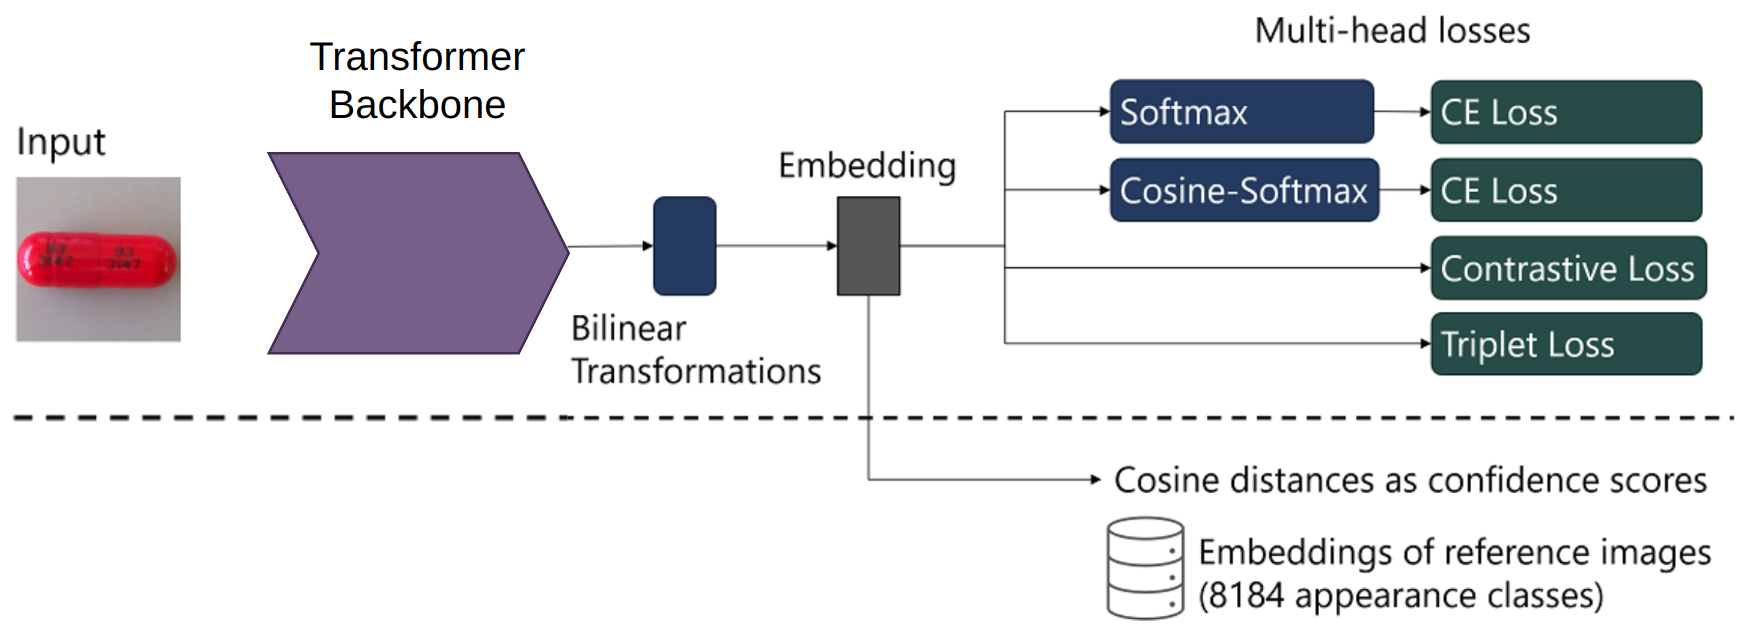
\includegraphics[width=.5\textwidth]{transformer-head.png}
    \caption{The architecture closely resembles the approach used by ~\cite{repo}. Instead of using a CNN backbone for feature extraction, we experiment with a Transformer.}
    \label{fig:t_head}
\end{figure}

\subsection{Losses}
The pill images in the dataset are structured in a way that they only ever appear once during training or testing, making this a complicated, few-shot classification task. To remedy this, we employ the multihead-loss implemented in~\cite{ePill}.  The loss is defined by:
\begin{equation}
L_{final} = \lambda_{SCE}L_{SCE} + \lambda_\eta L_\eta + \lambda_\rho L_\rho + \lambda_\Gamma L_\Gamma,
\end{equation}
where $L_{SCE}$ is a standard softmax cross-entropy loss, $L_\eta$ the arcface loss, $L_\rho$ the triplet loss, and $L_\Gamma$ the contrastive loss. The definitions of these are as follows:
\subsubsection{Arcface Loss}
\begin{equation}
L_\eta = -\log \frac{e^{s\cdot \text{cos}(\theta_{y_i})}}{e^{s\cdot \text{cos}(\theta_{y_i})} + \sum_{j=1, j\neq y_i}^N e^{s\cdot \text{cos}(\theta_j)}},
\end{equation}
where $\theta_{yi}$ is the angle between the weight vector $W_j$ of the true class $y_i$, and the feature $x_i$. $s$ is a scaling factor. The goal of $L_\eta$ is to maximize 
the margin and provide confidence scores between different classes. 
\subsubsection{Triplet Loss}
\begin{equation}
    L_\rho = \sum_{i=1}^{N}\left[\left||f\left(x_{i}^{a}\right)-f\left(x_{i}^{p}\right)\right||_{2}^{2}-\left||f\left(x_{i}^{a}\right)-f\left(x_{i}^{n}\right)\right||_{2}^{2}+\alpha\right]_{+},
\end{equation}
where $x_i^a$, $x_i^p$, and $x_i^n$ are the respective anchor, positive, and negative samples, and $f(\cdot)$ is an embedding function function. The goal of $L_\rho$ is to create an embedding space where $x_i^a$ and $x_i^p$ are closely related points in that space. Additionally, 
we want to maximize the distance between $x_i^a$ and $x_i^n$ in that space.
\subsubsection{Contrastive Loss}
\begin{equation}
L_\Gamma = \frac{1}{N} \sum_{i=1}^N \max(0, d_{pos} - d_{neg} + margin),
\end{equation}
where $d_{pos}$ are a postive examples, and $d_{neg}$ negative ones. With $L_\Gamma$, we take $d_{pos}$ and $d_{neg}$ as sample pairs, and our aim is to create a margin between the two sets of classes.
\subsection{Multi-Head Model}
In order to implement the triplet and contrastive losses, we need to add additional overhead to our embedded transformer architecture. 
To compare these two, we use the binary classifier head from ~\cite{repo} and pass the output $emb$ from the embedded model.  In the case of the arcface loss, a margin head is used in parallel, which also takes $emb$ as input, along with the target values.

\section{Experiments}
\begin{itemize}

    \item Different pre-processing techniques will be assessed. Some which will include various arrangements of image transformations, data normalization, and using different patch sizes.
    
    \item We will experiment with hyperparameter tuning in order to determine the most favorable set for this task.  Among these, we will test:

    \begin{itemize}
    
        \item A varying degree of transformer encoding blocks. 

        \item Using different activation functions.  We will consider activations like ReLU~\cite{relu2010} and GELU~\cite{gelu2016}, which are consistent with the standard architecture of Vision Transformers (ViTs)~\cite{an_imageworth}.  In addition to this, we will also look at the performance of classical approaches, such as Softmax~\cite{softmax}.

        
    \end{itemize}

    \item Our accuracies will then be compared with the CNN architecture used in~\cite{ePill}.
    % \item What you expect to discover from these experiments (for the proposal and milestone reports).
    % \item Your results and the analysis of those results (for milestone and final reports).
    % \item The datasets that you plan to use (along with a high-level overview of each dataset such as its size, annotations, when it was introduced, etc)
    % \item The motivation why those datasets are suitable for your project.
\end{itemize}

\section{Preliminary Analysis}

Compared to the results given in the paper this research is based on, our results fall behind in all of the metrics.   \par

\begin{table}[h]
    \begin{tabular}{@{}|ccccc|@{}}
    \toprule
    \multicolumn{1}{|c|}{Model}     & \multicolumn{1}{c|}{GAP}   & \multicolumn{1}{c|}{GAP@1} & \multicolumn{1}{c|}{MAP}   & MAP@1 \\ \midrule
    \multicolumn{5}{|c|}{\textbf{Multi-head Metric Learning: Both-sides input}}                                                    \\ \midrule
    \multicolumn{1}{|c|}{ResNet50}  & \multicolumn{1}{c|}{58.75} & \multicolumn{1}{c|}{80.26} & \multicolumn{1}{c|}{83.51} & 74.28 \\ \midrule
    \multicolumn{1}{|c|}{Swin\_v2*} & \multicolumn{1}{c|}{46.83} & \multicolumn{1}{c|}{71.54} & \multicolumn{1}{c|}{77.05} & 65.18 \\ \midrule
    \multicolumn{1}{|c|}{Swin\_v2}  & \multicolumn{1}{c|}{7.73}  & \multicolumn{1}{c|}{32.45} & \multicolumn{1}{c|}{28.67} & 15.65 \\ \bottomrule
    \end{tabular}
    \end{table}

\section{Future Plans}

As shown above we currently achieve what we consider a sub-par accuracy for identification. As a result, we would like to look into methods that can improve the robustness of our apporach. One approach we are considering in the future is the usage of data augmentation. For this task we plan to use pre-existing solution called Cs$^2$. Cs$^2$ is an approach that uses generative models to create data augmentations to an already-existing dataset \cite{cs2}. By incorporating this into our current pipeline we hope that it can allow our model to train and see more variation which can hopefully result in overall better accuracies.  \par

In addition to more powerful data augmentations, we also would like to look into improvements to training the SWIN model. This could involve the un-freezing of specific layers in order for the model to better fit the inputs. We may also investigate other models that may be applicable. This is an area we are actively looking into at the time of writing this. \par 

% \section*{References}

% You should also include references to previous work.



%\begin{figure*}
%\begin{center}
%\fbox{\rule{0pt}{2in} \rule{.9\linewidth}{0pt}}
%%\includegraphics[width=0.8\linewidth]{figure2.pdf}
%\end{center}
%   \caption{Optional detailed illustration of your approach.}
%\label{fig:fig2}
%\end{figure*}

% \begin{table}
% \begin{center}
% \begin{tabular}{c c}
% \hline
% Method & Accuracy \\
% \hline
% Theirs & 0.5 \\
% Yours & 0.75\\
% Ours & \bf 0.9 \\
% \hline
% \end{tabular}
% \end{center}
% \caption{Results for your milestone and final reports.}
% \end{table}




{\small
\bibliographystyle{unsrt}
\bibliography{sample}
}

\end{document}
